
%(BEGIN_QUESTION)
% Copyright 2007, Tony R. Kuphaldt, released under the Creative Commons Attribution License (v 1.0)
% This means you may do almost anything with this work of mine, so long as you give me proper credit

It is common in some digital networks to connect paralleled devices to the network cable, like this:

$$\includegraphics[width=15.5cm]{i02188x01.eps}$$

Note that the far-end devices have terminating resistors connected in parallel to the network connection terminals, while the devices at the end of the stubs do not.  Does this constitute a problem?  In other words, will reflected signals result from the unterminated stubs?  Why or why not?

Furthermore, what would happen if each of the stub devices were terminated with the same resistance value as the end devices?

\vskip 20pt \vbox{\hrule \hbox{\strut \vrule{} {\bf Suggestions for Socratic discussion} \vrule} \hrule}

\begin{itemize}
\item{} Supposing the cable's characteristic impedance is 100 $\Omega$, how much resistance should each of the terminating resistors in this network have?
\end{itemize}

\underbar{file i02188}
%(END_QUESTION)





%(BEGIN_ANSWER)

Lack of termination is not a problem so long as the stubs are short enough.  The same principle applies to the network as a whole: if the total cable length is short enough, no termination resistors are needed anywhere!

Terminating all devices in the network could be problematic due to signal loading.  With each additional termination resistor, the signal ``sees'' a heavier load.  Too much loading and the signal voltage could sag below compliance.

\vskip 10pt

Follow-up question \#1: how do we define ``short enough'' in this context?  How do we know if a cable (or stub) is long enough to require termination?

\vskip 10pt

Follow-up question \#2: how do we define ``compliance'' voltage levels for digital signals in this context?  How do we know if we will load down the signal too much with too many termination resistors in parallel?

%(END_ANSWER)





%(BEGIN_NOTES)

All unterminated cables produce signal reflections.  If the stubs are short enough, though, their reflected signals echo so fast back to the main pulse that it will not be noticeable.

``Short enough'' is defined as the length below which any glitches resulting from reflected signal interference becomes insignificant to the receiving devices.  This depends on the bit rate of the digital data (i.e. how long the normal digital pulses are).  If the regular pulse length is long enough to swamp out the reflected signal glitches that result from lack of termination, the network will function just fine.  Otherwise, these glitches will corrupt the digital data!

\vskip 10pt

You could terminate all cable stub ends, but all that resistance may place undue load on the signal itself, until its amplitude falls below the devices' compliance level.  This ``compliance'' voltage level is likewise defined by the receiving devices.  This is a similar question to the acceptable ``high'' and ``low'' signal levels for different logic gate families (CMOS, TTL, ECL, etc.), and may be answered by studying the manufacturer's datasheets.

%INDEX% Electronics review: characteristic impedance of transmission line
%INDEX% Electronics review: surge impedance of transmission line

%(END_NOTES)


